% SPDX-License-Identifier: CC-BY-4.0
%
% Copyright (c) 2024 Nelson Vieira and Mary Barreto
%
% @author Nelson Vieira <2080511@student.uma.pt>
% @contributor Mary Barreto <mary.barreto@staff.uma.pt>
% @license CC-BY-4.0 <https://creativecommons.org/licenses/by/4.0/legalcode.txt>
\documentclass[xcolor={svgnames},compress,aspectratio=169]{beamer}
\usetheme{Berlin}
\usecolortheme{dolphin}

\setbeamercolor*{structure}{bg=Azure,fg=MidnightBlue!50!black}

\setbeamercolor*{palette primary}{use=structure,fg=structure.bg,bg=structure.fg}
\setbeamercolor*{palette secondary}{use=structure,fg=structure.fg,bg=structure.bg}
\setbeamercolor*{palette tertiary}{use=structure,fg=structure.fg,bg=GhostWhite}
\setbeamercolor*{palette quaternary}{fg=white,bg=black}

\setbeamercolor{section in head/foot}{parent=palette primary} % Outer section of header/footer
\setbeamercolor{subsection in head/foot}{parent=palette secondary} % Inner section of header/footer

\setbeamercolor{titlelike}{parent=palette tertiary} % Main titles
\setbeamercolor{frametitle}{parent=palette tertiary,bg=GhostWhite!50}

\setbeamercolor{section in toc}{fg=darkgray,bg=Azure} % Table of contents sections
\setbeamercolor{subsection in toc}{fg=darkgray,bg=Azure} % Table of contents subsections
% \setbeamercolor{alerted text}{use=structure,fg=structure.fg!50!black!80!black}

% \setbeamertemplate{navigation symbols}{} % Hides navigation buttons at the bottom
% \setbeamertemplate{headline}{} % Hides navigation bar at the top

\setbeamercovered{transparent}

\setbeamertemplate{caption}[numbered]

% \usepackage{pgfpages}
% \pgfpagesuselayout{4 on 1}[a4paper,border shrink=5mm]

\usepackage[utf8]{inputenc}
\usepackage{adjustbox}
\usepackage{xcolor,colortbl}
\usepackage[all]{xy}
\usepackage{tikz}
\usetikzlibrary{mindmap,backgrounds}
\usepackage{graphicx}
\usepackage{multicol}
% Advanced table functions
\usepackage{tabularx,ragged2e}
\usepackage{booktabs}
% Listings extension
\usepackage{listings}
\usepackage{transparent}
\usepackage{amsmath,amssymb,amsfonts}
\usepackage[font=tiny]{caption}
\usepackage[font=tiny]{subcaption}
\usepackage{pgfplots}
\usepackage{pgf-pie}
\usepackage{tcolorbox}
\usepackage{svg}
\setsvg{inkscape = "C:/Program Files/Inkscape/bin/inkscape.exe"}
\svgsetup{inkscapepath=svgsubdir}
\def\myversion{0.5}

\title[Privacy and Digital Literacy in the Internet of Things]{{\normalsize 22nd International Conference e-Society 2024} \\ Privacy and Digital Literacy in the Internet of Things}
% \subtitle{}
\author{\href{mailto:2080511@student.uma.pt}{Nelson Vieira} and \href{mailto:mary.barreto@staff.uma.pt}{Mary Barreto}}
\institute[\href{https://www.uma.pt/}{University of Madeira}]{University of Madeira\\Faculty of Exact Sciences and Engineering}
\date{{\scriptsize Last Update: \today}}

\setbeameroption{hide notes}

\makeatletter
    \newenvironment{withoutheadline}{
        \setbeamertemplate{headline}[default]
        \def\beamer@entrycode{\vspace*{-\headheight}}
    }{}
\makeatother

\begin{document}

\begin{withoutheadline}
    \begin{frame}
        % \centering\includegraphics[width=90pt]{assets/images/uma_logo.png}
        \maketitle
    \end{frame}
\end{withoutheadline}

\begin{frame}{Table of Contents}
    % Use hideallsubsections for longer presentations
    % \tableofcontents[hideallsubsections]
    \begin{multicols}{2}
        \tableofcontents
    \end{multicols}
\end{frame}

\section{Introduction}

% Option [fragile] needed for lstlisting
\begin{frame}[fragile]
    \begin{multicols}{2}
        \centering
        % {\footnotesize What is privacy?}
        \begin{figure}
            \centering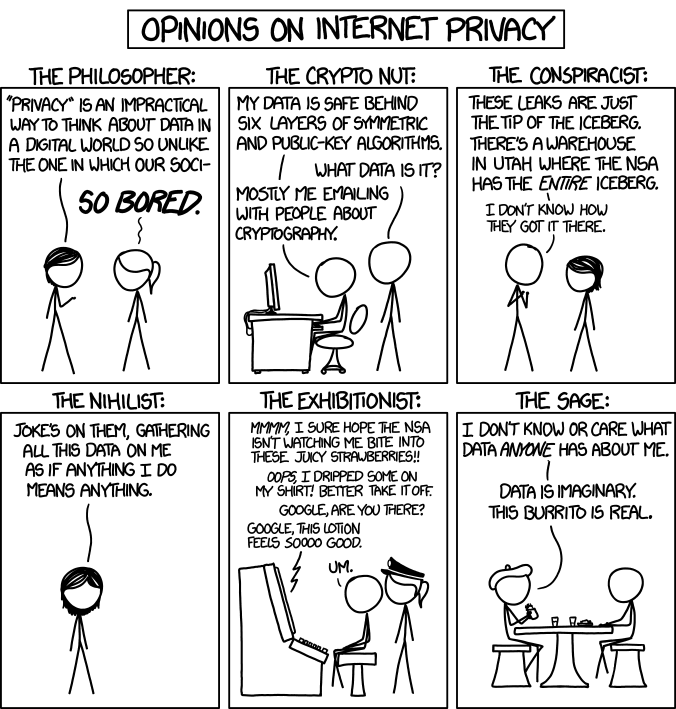
\includegraphics[width=155pt]{assets/images/privacy_opinions.png}\\
            \textcolor{gray}{{\tiny \textcopyright \href{https://xkcd.com/1269/}{Randall Munroe}, \href{https://creativecommons.org/licenses/by-nc/2.5/}{CC BY-NC 2.5 License}}}
        \end{figure}

        \columnbreak
        \vspace*{\fill}
\begin{lstlisting}[language=sh,escapechar=\%]
    diff privacy.c
    %\big\uparrow%     %\textcolor{blue}{@@ -1,1 +1,1 @@}%
    1 %\textcolor{red}{- Privacy}%
    1 %\textcolor{green!60!black!80}{+ Security}%
    %\big\downarrow%     ...
\end{lstlisting}
        \vspace*{\fill}
    \end{multicols}
\end{frame}

\note{
    There is some contention on the definition of privacy. Most literature assumes
    that privacy is equal to security or that it is only a part of it, as such
    by creating better security systems they assume to alse solve privacy problems.
    This work takes privacy on its own.
}

\begin{frame}{Introduction}
    The advent of ubiquitous computing has resulted in the widespread use of
    Internet of Things devices. These devices open up
    new avenues for the collection and exploitation of user and non-user personal
    data. Most end users are not even aware or have little control over the
    information that is being collected about them by these systems.

    % This work took a rounded approach to this problem.
    % \begin{itemize}
    %     \item<1-> Literature review;
    %     \item<2-> A survey.
    % \end{itemize}
\end{frame}

\note{
    This work tackles privacy literacy in IoT systems. An holistic approach was taken
    and consisted in doing a systematic literature review, a survey and a mobile application.
}

\section{State of the Art}

\begin{frame}{Privacy Paradox}
    \vspace*{\fill}
    It happens when the opinions stated by the users are radically different from their actions.

    \vspace*{\fill}
    Proven to be debased by a number of empirical studies \cite{sannon2018privacy,xie2019consumers}.
    \vspace*{\fill}
\end{frame}

\note{
    Why even worry about privacy if people seamingly do not care about it
    by their actions?
    This topic is more nuanced, people behave in ways that are not
    inherently paradoxical, they base their actions in various factors.
}

\begin{frame}{State of the Art}
    \vspace*{\fill}
    There are two main ways to provide privacy in IoT systems:
    \vspace*{\fill}
    \begin{itemize}
        \item[$\bullet$]<1->
        Through security \cite{zhao2020local, zhang2017privacy, ali2017iot};
        \item[$\bullet$]<2->
        User awareness (eg. privacy notices) \cite{feng2021design, das2018personalized};
    \end{itemize}
    \vspace*{\fill}
    Legislation or a framework/architecture mainly fall into one these two categories.
    \vspace*{\fill}
\end{frame}

\note{
    Most literature approaches fall under privacy through security.
    Very few approach privacy as a unique concept with its own characteristics.
    Privacy literacy is barely taken on.
}

\begin{frame}{State of the Art}
    Skirpan et al. (2022) \cite{skirpan2022is} developed an interactive theatre
    experience as a case study to gather user awareness about digital
    privacy.
    The authors
    noted that after contacting people months after the initial interviews
    that they did not really changed their behaviour regarding
    their privacy.

    \vspace*{\fill}
    The Carnegie Mellon University CyLab designed a personalized privacy
    assistant (2020) \cite{colnago2020informing} where users could see
    IoT devices near their location. The implementation is
    fragmented with the creation of an application \cite{feng2021design} the cannot
    be interacted with and a webpage \cite{das2018personalized} where users can actually modify data.
\end{frame}

\note{
    An interactive theatre experience was developed by (Skirpan et al., 2022)
    as a case study of an innovative approach to gather user awareness about
    their online behaviour regarding privacy. This was created to try to
    prove that a simulated experience with a credible privacy problem may
    encourage people to act before encountering a breach. The authors
    noted that after contacting people months after the initial interviews
    that they did not really changed their behaviour regarding their privacy.

    (Colnago et al., 2020) designed a personalized privacy assistant
    (PPA) and conducted interviews to examine user perceptions of
    hypothetical PPA implementations. The authors found that the
    participants' attitudes regarding the various implementations
    were generally favourable, although they also voiced worries,
    which varied depending on the degree of automation. After the
    design phase, a privacy assistant (Feng, Yao and Sadeh, 2021)
    was developed using a notice and choice approach. The application
    is not capable of identifying new IoT devices, users have to add
    new devices on a webpage (Das et al., 2018).
}

\section{Methodology}

\subsection{Survey}

\begin{frame}[shrink]{Survey}
    \begin{multicols}{2}
        86 Questions
        \begin{itemize}
            \item General knowledge and attitudes towards privacy
            \item Disposition for sharing personal information
            \item Privacy concerns
            \item Current online habits and practices
            \item Profile identification
            \item Knowledge and habits regarding the Internet of Things
            \item Demographic data
        \end{itemize}

        \columnbreak
        \vspace*{\fill}
        \begin{figure}
            \centering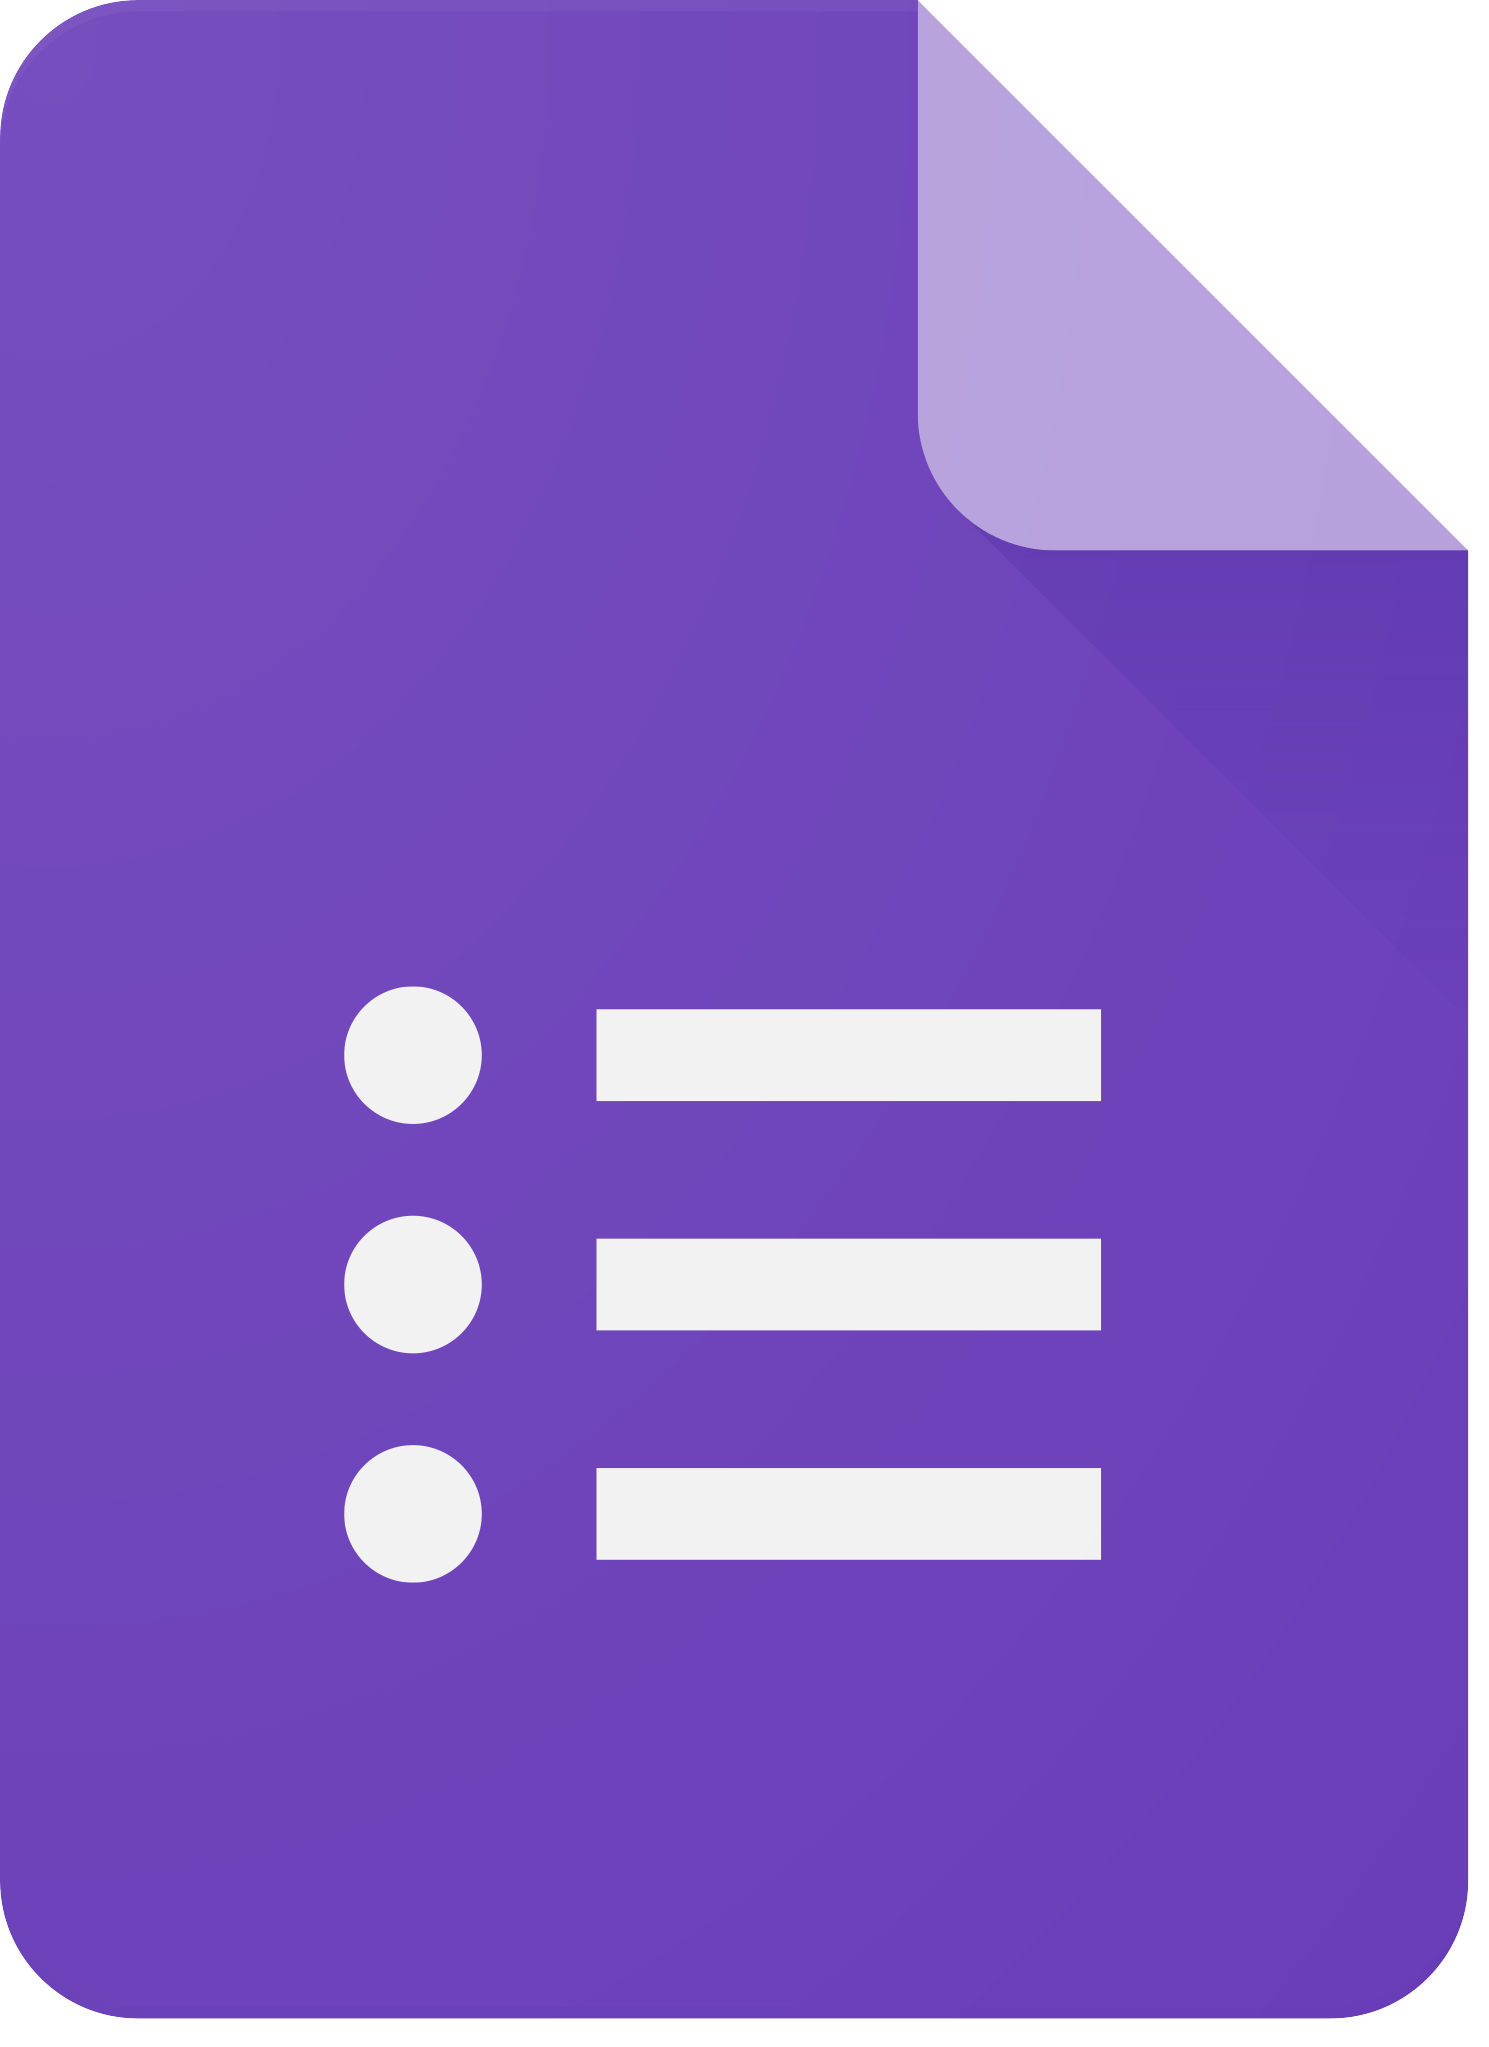
\includegraphics[width=45pt]{assets/images/forms.png}\\
            \textcolor{gray}{{\tiny Google Forms, \href{https://www.google.com/images/about/forms-icon.svg}{https://www.google.com/images/about/forms-icon.svg}}}
        \end{figure}
        \vspace*{\fill}
    \end{multicols}
\end{frame}

\note{
    Survey with varied questions from general privacy concerns to online habits and IoT literacy.
    86 questions under 7 main topics of interest from privacy attitudes, concerns, online habits to IoT knowledge and usage.
}

\begin{frame}
    \begin{multicols}{2}
        \begin{figure}
            \adjustbox{minipage=1.3em,valign=t}{\subcaption{}\label{sfig:survey_privacy_importance}}%
            \begin{subfigure}[t]{0.45\textwidth}
                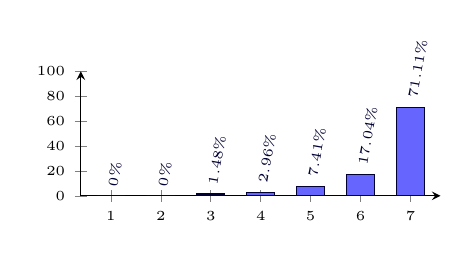
\begin{tikzpicture}
                    \begin{axis}[
                        width=175pt,
                        height=90pt,
                        ybar,
                        bar width=10pt,
                        ymin=0,
                        ymax=100,
                        xtick=data,
                        xtick style={font=\tiny},
                        ytick style={font=\tiny},
                        xtick style={font=\tiny},
                        ytick style={font=\tiny},
                        xticklabel style={font=\tiny},
                        yticklabel style={font=\tiny},
                        ylabel style = {font=\tiny},
                        xlabel style = {font=\tiny},
                        axis x line=bottom,
                        axis y line=left,
                        enlarge x limits=0.1,
                        nodes near coords={\pgfmathprintnumber\pgfplotspointmeta\%},
                        every node near coord/.append style={rotate=80, anchor=west, font=\tiny},
                        legend style={at={(0.5,-0.1)},anchor=north}
                    ]
                        \addplot[blue!20!black,fill=blue!60!white] coordinates {(1,0) (2,0) (3,1.48) (4,2.96) (5,7.41) (6,17.04) (7,71.11)};
                    \end{axis}
                \end{tikzpicture}
                % \caption{}
                % \label{fig:survey_privacy_importance}
            \end{subfigure}
            \adjustbox{minipage=1.3em,valign=t}{\subcaption{}\label{sfig:survey_it_terms}}%
            \begin{subfigure}[t]{0.45\textwidth}
                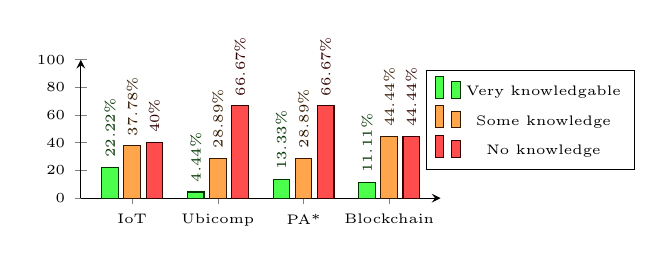
\begin{tikzpicture}
                    \begin{axis}[
                        width=175pt,
                        height=95pt,
                        symbolic x coords={IoT,Ubicomp,PA*,Blockchain},
                        ybar,
                        bar width=6pt,
                        ymin=0,
                        ymax=100,
                        xtick style={font=\tiny},
                        ytick style={font=\tiny},
                        xtick style={font=\tiny},
                        ytick style={font=\tiny},
                        xticklabel style={font=\tiny},
                        yticklabel style={font=\tiny},
                        ylabel style = {font=\tiny},
                        xlabel style = {font=\tiny},
                        axis x line=bottom,
                        axis y line=left,
                        enlarge x limits=0.2,
                        nodes near coords={\pgfmathprintnumber\pgfplotspointmeta\%},
                        every node near coord/.append style={rotate=90, anchor=west, font=\tiny},
                        legend style={at={(1.25,0.20)},anchor=south}
                    ]
                        \addplot[green!20!black,fill=green!70!white] coordinates {(IoT,22.22) (Ubicomp,4.44) (PA*,13.33) (Blockchain,11.11)};
                        \addlegendentry{{\tiny Very knowledgable}}
                        \addplot[orange!20!black,fill=orange!70!white] coordinates {(IoT,37.78) (Ubicomp,28.89) (PA*,28.89) (Blockchain,44.44)};
                        \addlegendentry{{\tiny Some knowledge}}
                        \addplot[red!20!black,fill=red!70!white] coordinates {(IoT,40) (Ubicomp,66.67) (PA*,66.67) (Blockchain,44.44)};
                        \addlegendentry{{\tiny No knowledge}}
                    \end{axis}
                \end{tikzpicture}
                % \caption{}
                % \label{fig:survey_it_terms}
            \end{subfigure}
            \caption{{\tiny Participant responses regarding: (a) participants' privacy importance perception and (b) general IT knowledge. (Section 4)}}
            \label{fig:survey_responses_privacy_importance_it_terms}
        \end{figure}

        \columnbreak
        % \hspace{0.2\linewidth}
        \begin{itemize}
            \item[$\bullet$]
            High regard for privacy, with some caveats;
            \item[$\bullet$]
            Some difficulty understating digital privacy;
            % \item[$\bullet$]
            % Different attitudes with different systems;
            \item[$\bullet$]
            Low literacy of technical jargon;
        \end{itemize}
        \vspace{1cm}
        \begin{flushright}
            {\tiny *PA - Privacy Assistant}
        \end{flushright}
    \end{multicols}
\end{frame}

\note{
    Majority of respondents found that privacy is very important.
    But lack knowledge about IoT and more esoteric IT or privacy topics.
}

\begin{frame}
    \begin{multicols}{2}
        \begin{figure}
            \begin{subfigure}[t]{0.45\textwidth}
                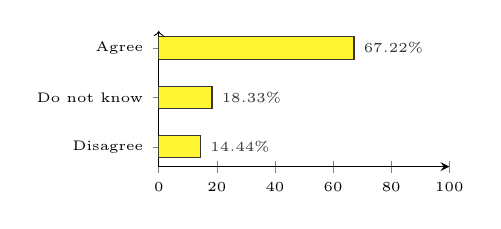
\begin{tikzpicture}
                    \begin{axis}[
                        width=150pt,
                        height=95pt,
                        xbar,
                        symbolic y coords={Disagree,Do not know,Agree},
                        bar width=8pt,
                        ytick=data,
                        axis x line=bottom,
                        axis y line=left,
                        xtick style={font=\tiny},
                        ytick style={font=\tiny},
                        xtick style={font=\tiny},
                        ytick style={font=\tiny},
                        xticklabel style={font=\tiny},
                        yticklabel style={font=\tiny},
                        ylabel style = {font=\tiny},
                        xlabel style = {font=\tiny},
                        xmin=0,
                        xmax=100,
                        enlarge y limits=0.2,
                        y axis line style={->,shorten >=1pt},
                        nodes near coords={\pgfmathprintnumber\pgfplotspointmeta\%},
                        every node near coord/.append style={font=\tiny},
                        legend style={at={(0.5,-0.1)},anchor=north, font=\tiny}
                    ]
                        \addplot[yellow!10!black,fill=yellow!80!white] coordinates {(14.44,Disagree) (18.33,Do not know) (67.22,Agree)};
                    \end{axis}
                \end{tikzpicture}
                {\tiny\caption{}}
                \label{fig:survey_privacy_notices}
            \end{subfigure}
            \begin{subfigure}[t]{0.45\textwidth}
                    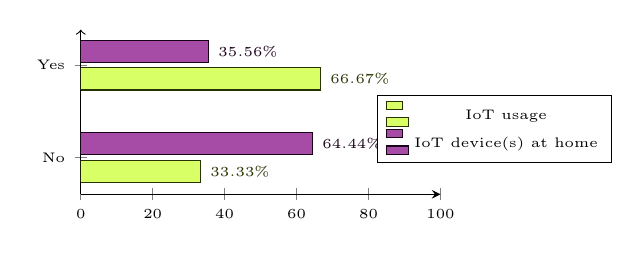
\begin{tikzpicture}
                        \begin{axis}[
                            width=175pt,
                            height=105pt,
                            xbar,
                            symbolic y coords={No,Yes},
                            bar width=8pt,
                            ytick=data,
                            xtick style={font=\tiny},
                            ytick style={font=\tiny},
                            xtick style={font=\tiny},
                            ytick style={font=\tiny},
                            xticklabel style={font=\tiny},
                            yticklabel style={font=\tiny},
                            ylabel style = {font=\tiny},
                            xlabel style = {font=\tiny},
                            axis x line=bottom,
                            axis y line=left,
                            xmin=0,
                            xmax=100,
                            enlarge y limits=0.4,
                            y axis line style={->,shorten >=0.5pt},
                            nodes near coords={\pgfmathprintnumber\pgfplotspointmeta\%},
                            every node near coord/.append style={font=\tiny},
                            legend style={at={(1.15,0.60)},anchor=north}
                        ]
                            \addplot[lime!20!black,fill=lime!60!white] coordinates {(33.33,No) (66.67,Yes)};
                            \addlegendentry{{\tiny IoT usage}}
                            \addplot[violet!20!black,fill=violet!70!white] coordinates {(64.44,No) (35.56,Yes)};
                            \addlegendentry{{\tiny IoT device(s) at home}}
                        \end{axis}
                    \end{tikzpicture}
                    {\tiny\caption{}}
                    \label{fig:internet_of_things_device_usage}
            \end{subfigure}
            \caption{Participant responses regarding: (a) unwillingness to read privacy notices and (b) IoT usage. (Section 4)}
            \label{fig:survey_responses_privacy_notices_iot_usage}
        \end{figure}

        \columnbreak
        \hspace*{\fill}
        \begin{itemize}
            \item[$\bullet$]
            Dismissal of privacy notices due to various factors;
            \item[$\bullet$]
            Some individuals (55\%) use fake private data online;
            \item[$\bullet$]
            Some interaction with Internet of Things devices but low knowledge generally;
            \item[$\bullet$]
            Low grasp of IoT privacy;
        \end{itemize}
        \hspace*{\fill}
    \end{multicols}
\end{frame}

\note{
    Some notes here.
}

\section{Conclusion and Future Work}

\subsection{Future Work}

\begin{frame}{Limitations and Future Work}
    Survey limitations:
    \begin{itemize}
        \item[$\bullet$]
        Too dense;
        \item[$\bullet$]
        Limited number of participants.
    \end{itemize}
    Topics for further research:
    \begin{itemize}
        \item[$\bullet$]
        Privacy literacy in IoT systems;
        \item[$\bullet$]
        Application of privacy in the design/development of IoT systems;
        \item[$\bullet$]
        User-centric approaches to IoT privacy.
    \end{itemize}
\end{frame}

\note{
    Some notes here.
}

\subsection{Conclusion}

\begin{frame}{Conclusion}
    \begin{itemize}
        \item[$\bullet$]
        Results from majority viewpoint of portuguese participants;
        \item[$\bullet$]
        Survey results reveal that there is a large privacy knowledge gap;
        \item[$\bullet$]
        There should be more tools focused on privacy literacy.
    \end{itemize}
\end{frame}

\note{
    This work contributed to the overall body of research by compiling and reviewing
    other works with the perspective of privacy as a distinct subject matter rather than
    an extension of security, as many publications imply. The survey conducted
    on the perception of individuals on privacy in IoT systems portrays the majority
    viewpoint of portuguese people, since 60\% of participants were portuguese.
}

\begin{frame}
    \begin{center}
        {\large Thank you for your attention.}
    \end{center}
\end{frame}

\section*{References}

\begin{frame}[allowframebreaks]{References}
    \bibliographystyle{IEEEtran}
    {\footnotesize \bibliography{assets/references}}
\end{frame}

\end{document}
